
% 0. Many methods for electronic structure calculations
% tradeoffs between accuracy and cost scaling
% want to compare results from different methods
% DMC is a "good deal" for electronic calculations

\begin{frame}{Electronic structure methods}
\vspace{2em}
\begin{minipage}{.26\textwidth}
multiple techniques:
\begin{itemize}[leftmargin=1em, itemsep=1ex, label=-]
\item tradeoff: 

cost vs accuracy
\item different situations 
\item validation on the same problem
\end{itemize}
\end{minipage}
\end{frame}

\begin{frame}{Electronic structure methods}
\begin{minipage}{.26\textwidth}
multiple techniques:
\begin{itemize}[leftmargin=1em, itemsep=1ex, label=-]
\item tradeoff: 

cost vs accuracy
\item different situations 
\item validation on the same problem
\end{itemize}

\vspace{1em}
diffusion Monte Carlo is a good deal!

\vspace{1em}
\parbox{\textwidth}{\tiny K.T. Williams, et. al., Phys. Rev. X 10, 011041, (2020).}
\end{minipage}
\hspace{.03\textwidth}
\begin{minipage}{.65\textwidth}
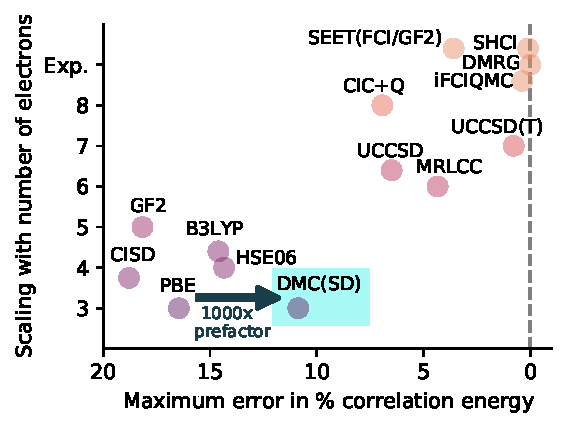
\includegraphics[width=\textwidth]{figures/scaling_vs_energy.pdf}
\end{minipage}
\end{frame}


% Pre-1: what is DMC
\begin{frame}{Diffusion Monte Carlo: projection onto ground state}

\begin{minipage}[t]{.45\textwidth}
\vspace{-1em}
\begin{itemize}[leftmargin=0em]
\item apply $e^{-\hat{H}t}$ to trial function $|\Psi_T\rangle$
\item $t\rightarrow\infty$
\item higher eigenstates suppressed
\end{itemize}

\pagehline

Expansion in eigenstates
\vspace{-1ex}
\begin{align*}
|\Psi_T\rangle &= c_0 |\Phi_0\rangle + c_1 |\Phi_1\rangle + \ldots \\
e^{-\hat{H}t}|\Psi_T\rangle &= c_0 e^{-E_0t}|\Phi_0\rangle + c_1  e^{-E_1t}|\Phi_1\rangle + \ldots
\end{align*}
\end{minipage}
\end{frame}

\begin{frame}{Diffusion Monte Carlo: projection onto ground state}

\begin{minipage}[t]{.45\textwidth}
\vspace{-1em}
\begin{itemize}[leftmargin=0em]
\item apply $e^{-\hat{H}t}$ to trial function $|\Psi_T\rangle$
\item $t\rightarrow\infty$
\item higher eigenstates suppressed
\end{itemize}

\pagehline

Expansion in eigenstates
\vspace{-1ex}
\begin{align*}
|\Psi_T\rangle &= c_0 |\Phi_0\rangle + c_1 |\Phi_1\rangle + \ldots \\
e^{-\hat{H}t}|\Psi_T\rangle &= c_0 e^{-E_0t}|\Phi_0\rangle + c_1  e^{-E_1t}|\Phi_1\rangle + \ldots
\end{align*}

\pagehline

Approximations:

\begin{itemize}[leftmargin=1em]
\item fixed nodes $\Psi_T(R) = 0 \rightarrow \Psi(R) = 0$
\item localize nonlocal pseudopotentials
\end{itemize}
$\rightarrow$ need good trial function $\Psi_T$
\end{minipage}
\begin{minipage}[t]{.45\textwidth}
Random walk $R_1 \rightarrow R_2 \rightarrow \ldots$

\begin{align*}
e^{-\hat{H}t}|\Psi_T\rangle = \int & dR_1 \ldots dR_N
\\& e^{-\hat{H}\tau}|R_N\rangle\langle R_N|
\\&\ldots
\\& e^{-\hat{H}\tau}|R_2\rangle\langle R_2|
\\& e^{-\hat{H}\tau}|R_1\rangle\langle R_1|\Psi_T\rangle 
\end{align*}


\end{minipage}

\end{frame}

% 2. explain vmc and dmc
% Create a trial function, e.g. Slater determinant times Jastrow function (of electron distances)
% VMC evaluates \langle \Psi | O | \Psi \rangle (e.g. energy)
% can optimize parameters to minimize vmc energy
% DMC projects the trial function onto the ground state,  e^{-\beta H} |\Psi_T\rangle
\begin{frame}{QMC trial function}
\begin{minipage}[t]{0.45\textwidth}
\begin{center}
\textbf{Trial function}
\end{center}

{\footnotesize
\vspace{1em}
A many-body ``guess'' to start the QMC calculation
\[\Psi_T(R) = \Psi_S(R) e^{J(R)}\]

\pagehline

%
%\color{darkgray}{
\vspace{1ex}

Slater determinant $\Psi_S(R)$

\vspace{1ex}
%
%\[\Psi_S(R) = \det\lbrace \phi_i(r_j) \rbrace\]
%orbitals $\phi_i$, electrons at $r_j$:
%
%or multi-Slater combination
%\[\Psi_{MS}(R) = \sum_n c_n \Psi_{S,n}(R)\]
%
Jastrow factor $e^{J(R)}$ 

\vspace{1ex}
%depends on pair distances (e-e and e-ion)%$r_{ij}$ and $r_{iI}$ (e-ion).
%\begin{itemize}[leftmargin=1em, itemsep=-1ex, label=-]
%\item electrons avoid each other
%\item cusp conditions
%\end{itemize}
%}

$R$: \parbox[t]{.8\textwidth}{$3N$ positions of all $N$ electrons}

}
\end{minipage}
\hspace{.02\textwidth}
\begin{minipage}[t]{0.45\textwidth}
\begin{center}
\textbf{Variational Monte Carlo (VMC)}
\end{center}

{\footnotesize 
\vspace{1em}
Goal: \parbox[t]{.7\textwidth}{evaluate $\langle\hat{O}\rangle_{\Psi_T}$ for operator $\hat{O}$ }

\vspace{1em}

\[\langle\hat{O}\rangle = \frac{\langle \Psi_T | \hat{O} | \Psi_T \rangle}
{\langle \Psi_T | \Psi_T \rangle}
\]

Sample $|\Psi_T|^2$ by random walk

and average estimator for $\hat{O}$
\vspace{1em}

$\rightarrow$ use $\langle\hat{H}\rangle_{\Psi_T}$ to {optimize parameters} of $\Psi_T$
%\pagehline

%\color{darkgray}{
%Method:
%\begin{itemize}[leftmargin=1em, itemsep=-1ex, label=-]
%\item sample $R$ from $|\Psi_T(R)|^2$
%\item average estimator 
%
%$\langle O_L(R)\rangle = 
%\left\langle \frac{O\Psi_T(R)}{\Psi_T(R)} \right\rangle$.
%\end{itemize}
%
%}
}
\end{minipage}
\end{frame}




% 1. workflow diagram
% Start with a mean-field or multi-determinant calculation to make trial function
% Optimize wf parameters using VMC energy and gradients
% Evaluate accumulators using VMC and DMC
\begin{frame}{Typical DMC workflow}
\begin{minipage}{\textwidth}
  \begin{center}
  \begin{tikzpicture}[>=stealth, thick]

\node(pyscf) [rectangle, draw, fill=blue!5!white, minimum width=5cm, minimum height=1.5cm]{\parbox{8cm}{\centering mean-field or multi-determinant calculation 

e.g. HF, DFT, CISD, CASCI
}};

%\node(scfdata) [below=1cm of pyscf, rectangle, draw, fill=cyan!20!white, minimum width=3cm]{cell, orbitals};

\node(optimize) [below=9mm of pyscf, rectangle, draw, fill=green!10!white, minimum width=5cm, minimum height=1.5cm]{\parbox{4cm}{\centering {\bf OPTIMIZE $\Psi$} \\ adjust parameters to minimize $\langle \Psi | H | \Psi \rangle$}};

%\node(wf)[below=1cm of optimize, rectangle, draw, fill=cyan!20!white, minimum width=4cm]{\parbox{2cm}{\centering trial wave function}};

%\node(vmc) [below left=9mm and 5mm of optimize.south, anchor=north east, rectangle, draw, fill=green!10!white, minimum width=3.5cm, minimum height=2.0cm]{\parbox{5.0cm}{\centering {\bf VMC} \\ average quantities $\langle\Psi|O|\Psi\rangle$ over optimized $\Psi$}};
\node(dmc) [below =9mm of optimize.south, anchor=north, rectangle, draw, fill=green!10!white, minimum width=3.5cm, minimum height=2.0cm]{\parbox{5.0cm}{\centering {\bf DMC} \\ average quantities $\langle\Psi|O|\Phi_0\rangle$ with projected ground state $\Phi_0$}};

\draw[->] (pyscf) -- 
%node [right=1cm, ellipse, draw=gray, fill=cyan!10!white, minimum width=2cm]{cell, orbitals} 
(optimize);
%\draw[->] (optimize) -- (vmc);
\draw[->] (optimize) -- 
%node[right=5mm, ellipse, draw=gray, fill=cyan!10!white, minimum width=2.2cm]{\parbox{2cm}{\centering optimized parameters}} 
(dmc);
\end{tikzpicture}



  \end{center}
\end{minipage}
\end{frame}


% 4. example code benzene
% PySCF cell
% PySCF mf
% supercell
% OPTIMIZE
% VMC
% DMC
\newcommand{\mycode}[1]{
\vspace{-1em}
%\begin{center}
\begin{minipage}[c]{.45\textwidth}
\lstinputlisting[language=Python]{#1}
\end{minipage}
%\end{center}
}

\newcommand{\mygraphic}[1]{
\begin{minipage}[c]{.48\textwidth}
\includegraphics[width=\textwidth]{#1}
\end{minipage}
}

\begin{frame}{Example: Benzene molecule}
\vspace{1em}
\begin{minipage}{1.05\textwidth}
\begin{minipage}[t]{0.35\textwidth}
{\bf HF with PySCF}
\lstinputlisting[language=Python]{snippets/fig_benzene_scf.py}

\vspace{1em}
{\footnotesize can also do periodic systems}

\end{minipage}
\hspace{2em}
\begin{minipage}[t]{0.58\textwidth}
{\bf PyQMC recipes}

\vspace{1em}
\mycode{snippets/fig_optimize_recipe.py}
\mygraphic{figures/benzene_linemin.pdf}

\vspace{1em}
\mycode{snippets/fig_vmc_and_dmc_recipe_lines.py}
\mygraphic{figures/benzene_both.pdf}

%\vspace{1em}
%\mycode{snippets/fig_dmc_recipe.py}
%\mygraphic{figures/h2o_dmc.pdf}

\end{minipage}
\end{minipage}

\end{frame}






% Performance
\begin{frame}{Code profile}
\begin{minipage}{.45\textwidth}
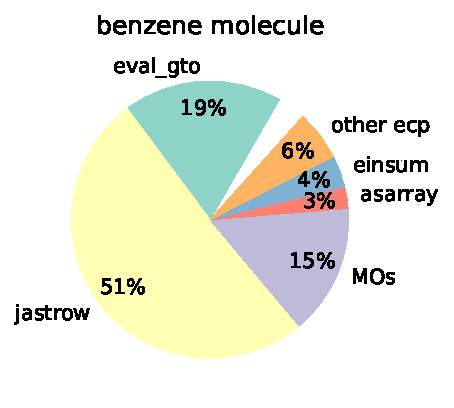
\includegraphics[height=.45\textheight]{figures/profile_benzene.pdf}

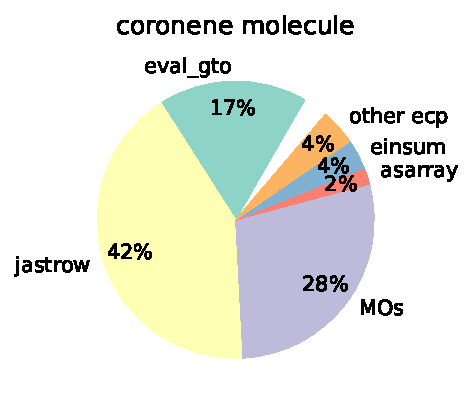
\includegraphics[height=.45\textheight]{figures/profile_coronene.pdf}
\end{minipage}
\hspace{.02\textwidth}
\begin{minipage}{.45\textwidth}
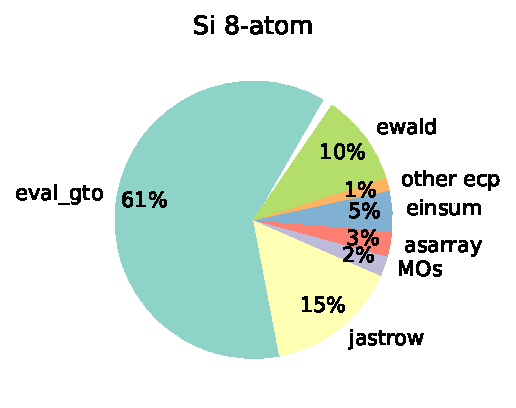
\includegraphics[height=.45\textheight]{figures/profile_Si1.pdf}

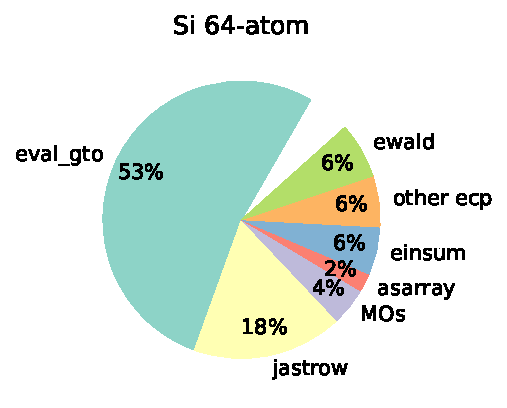
\includegraphics[height=.45\textheight]{figures/profile_Si2.pdf}
\end{minipage}
\end{frame}




% How it works: flowchart of VMC
% Running VMC

\begin{frame}%{Running VMC}
\begin{tikzpicture}[
    >=triangle 60,
    start chain=going below,
    node distance=3mm and 3mm,
    every join/.style={black, ->},
]
\scriptsize
\tikzset{
  box1/.style={rectangle, minimum height=8cm},
  box2/.style={draw, rectangle, rounded corners, minimum width=4cm},
  base/.style={draw, align=center, minimum height=2ex},
  flowelement/.style={base, fill=yellow!10!white, on chain, on grid, rectangle, rounded corners, aspect=3, text width=8em, inner sep=1mm},
  offchain/.style={base, rectangle, rounded corners, fill=yellow!10!white, text width=8em},
  % coord node style is used for placing corners of connecting lines
  coord/.style={rectangle, minimum height=2ex},
  % -------------------------------------------------
  % Connector line styles for different parts of the diagram
  it/.style={font={\small\itshape}}
}

% Containers
\node (cpubox) [box1, draw, fill=blue!5!white, minimum width=9.0cm]{};
\node (gpubox) [box1, right=of cpubox, fill=white!5!white, minimum width=5cm]{};

% VMC elements
\node (vmcbox) [box2, below right=of cpubox.north west, minimum height=4.5cm, fill=magenta!10!white]{};
\node (mclabel) [below=.8ex of vmcbox.north] {Monte Carlo steps};
\node (gradpsi) [flowelement, below=.8ex of mclabel.south, draw=cyan, thick]{compute $\nabla\Psi(R)$};
\node (proposemove) [flowelement, join]{propose  move $R\rightarrow R'$};
\node (gradpsi2) [flowelement, join, draw=cyan, thick]{compute $\Psi(R'), \nabla\Psi(R')$};
\node (acceptmove) [flowelement, join]{accept move $P_{\rm accept}(R\rightarrow R')$};

% Energy elements
\node (energybox) [box2, below=of vmcbox, minimum height=2.8cm, fill=magenta!10!white]{};
\draw[->] (vmcbox) -- (energybox);
\node (energylabel) [below=.8ex of energybox.north] {Energy};
\node (kinetic) [offchain, below=.8ex of energylabel, draw=cyan, thick]{kinetic $\nabla^2\Psi(R)$};
\node (ecp) [offchain, below=1ex of kinetic, draw=cyan, thick]{ECP $\Psi(\widetilde{R})$};
\node (potential) [offchain, below=1ex of ecp]{Coulomb/Ewald};


% WF elements
\node (wfbox) [box2, right=of vmcbox.north east, anchor=north west, minimum height=7cm, fill=cyan!10!white]{};
\node (slater) [below=.8ex of wfbox.north]{Slater};
\node (slatergrad) [offchain, below=.8ex of slater]{\texttt{eval\textunderscore gto} (AOs)};
\node (mos) [offchain, below=of slatergrad]{MOs};
\node (dets) [offchain, below=of mos]{determinant ratios};
\draw[->] (slatergrad) -- (mos);
\draw[->] (mos) -- (dets);

\node (jastrow) [below=3cm of slater]{Jastrow};
\node (dist) [offchain, below=.8ex of jastrow]{ee, ei distances};
\node (basis) [offchain, below=of dist]{\parbox{8em}{basis functions \\ ei: $a(r_{iI}), \nabla a(r_{iI})$ \\ ee: $b(r_{ij}), \nabla b(r_{ij})$}};
\draw[->] (dist) -- (basis);


% Labels
\node (cpulabel) [above=.8ex of cpubox]{CPU};
%\node (gpulabel) [above=.8ex of gpubox]{GPU};

% lines
\draw[-, cyan!70!black] (gradpsi.east) -- (wfbox.west);
\draw[-, cyan!70!black] (gradpsi2.east) -- (wfbox.west);
\draw[-, cyan!70!black] (kinetic.east) -- (wfbox.west);
\draw[-, cyan!70!black] (ecp.east) -- (wfbox.west);
\end{tikzpicture}
\end{frame}


\begin{frame}%{Running VMC on GPU}
\begin{tikzpicture}[
    >=triangle 60,
    start chain=going below,
    node distance=3mm and 3mm,
    every join/.style={black, ->},
]
\scriptsize
\tikzset{
  box1/.style={rectangle, minimum height=8cm},
  box2/.style={draw, rectangle, rounded corners, minimum width=4cm},
  base/.style={draw, align=center, minimum height=2ex},
  flowelement/.style={base, fill=yellow!10!white, on chain, on grid, rectangle, rounded corners, aspect=3, text width=8em, inner sep=1mm},
  offchain/.style={base, rectangle, rounded corners, fill=yellow!10!white, text width=8em},
  % coord node style is used for placing corners of connecting lines
  coord/.style={coordinate, on chain, on grid, node distance=6mm and 25mm},
  % -------------------------------------------------
  % Connector line styles for different parts of the diagram
  it/.style={font={\small\itshape}}
}

% Containers
\node (cpubox) [box1, draw, fill=blue!5!white, minimum width=9.0cm]{};
\node (gpubox) [box1, draw, right=of cpubox, fill=green!5!white, minimum width=5cm]{};

% VMC elements
\node (vmcbox) [box2, below right=of cpubox.north west, minimum height=4.5cm, fill=magenta!10!white]{};
\node (mclabel) [below=.8ex of vmcbox.north] {Monte Carlo steps};
\node (gradpsi) [flowelement, below=.8ex of mclabel.south, draw=cyan, thick]{compute $\nabla\Psi(R)$};
\node (proposemove) [flowelement, join]{propose  move $R\rightarrow R'$};
\node (gradpsi2) [flowelement, join, draw=cyan, thick]{compute $\Psi(R'), \nabla\Psi(R')$};
\node (acceptmove) [flowelement, join]{accept move $P_{\rm accept}(R\rightarrow R')$};

% Energy elements
\node (energybox) [box2, below=of vmcbox, minimum height=2.8cm, fill=magenta!10!white]{};
\draw[->] (vmcbox) -- (energybox);
\node (energylabel) [below=.8ex of energybox.north] {Energy};
\node (kinetic) [offchain, below=.8ex of energylabel, draw=cyan, thick]{kinetic $\nabla^2\Psi(R)$};
\node (ecp) [offchain, below=1ex of kinetic, draw=cyan, thick]{ECP $\Psi(\widetilde{R})$};
\node (potential) [offchain, below=1ex of ecp, draw=gray]{\color{gray}Coulomb};
\node (ewald) at (potential.east -| gpubox.north) [offchain, draw=gray]{Ewald};
\draw[->, thick, green!70!black] (energybox.east |- ewald.center) -- (ewald);


% WF elements
\node (wfbox) [box2, right=of vmcbox.north east, anchor=north west, minimum height=7cm, fill=cyan!10!white]{};
\node (slater) [below=.8ex of wfbox.north]{Slater};
\node (slatergrad) [offchain, below=.8ex of slater]{\texttt{eval\textunderscore gto} (AOs)};
\node (moscoord) [coord, below=of slatergrad]{};
\node (detscoord) [coord, below=of moscoord]{};
\node (mos) at (moscoord -| gpubox.north) [offchain] {MOs};
\node (dets) [offchain, below=of mos]{determinant ratios};
\draw[->, thick, green!70!black] (slatergrad) -- (mos);
\draw[->] (mos) -- (dets);
%\draw[->] (dets) -- (detscoord);

\node (jastrow) [below=3cm of slater]{Jastrow};
\node (jastcoord) [coord, below=1.8ex of jastrow]{};
\node (distcoord) [coord, below=1.8ex of jastcoord]{};
\node (dist) at (distcoord -| gpubox.north) [offchain]{ee, ei distances};
\node (basis) [offchain, below=of dist]{\parbox[c]{8em}{basis functions \\ ei: $a(r_{iI}), \nabla a(r_{iI})$ \\ ee: $b(r_{ij}), \nabla b(r_{ij})$}};
\draw[->] (dist) -- (basis);
\draw[->, thick, green!70!black] (jastcoord) -- (dist);
%\draw[->] (basis) -- (basis -| jastcoord);


% Labels
\node (cpulabel) [above=.8ex of cpubox]{CPU};
\node (gpulabel) [above=.8ex of gpubox]{GPU};

% lines
\draw[-, cyan!70!black] (gradpsi.east) -- (wfbox.west);
\draw[-, cyan!70!black] (gradpsi2.east) -- (wfbox.west);
\draw[-, cyan!70!black] (kinetic.east) -- (wfbox.west);
\draw[-, cyan!70!black] (ecp.east) -- (wfbox.west);
\end{tikzpicture}
\end{frame}


% CuPy
\begin{frame}{GPU implementation with CuPy}

\vspace{1em}

\begin{minipage}{0.93\textwidth}
\begin{itemize}[leftmargin=0em, itemsep=1em]
\item GPU with CuPy$^*$ library \texttt{https://cupy.dev}

\quad  uses NumPy interface 
\item minimal code changes 

\quad same code with CPU/GPU
\item still optimizing performance
\end{itemize}

\vspace{1em}
\parbox{\textwidth}{\tiny $^*$Ryosuke Okuta, Yuya Unno, Daisuke Nishino, Shohei Hido and Crissman Loomis. CuPy: A NumPy-Compatible Library for NVIDIA GPU Calculations. Proceedings of Workshop on Machine Learning Systems (LearningSys) in The Thirty-first Annual Conference on Neural Information Processing Systems (NIPS), (2017).}
\end{minipage}

\end{frame}

% 6. GPU performance
% VMC on small hydrocarbon molecules
% GPU is a big reduction as nelec becomes large (many systems of interest)
\begin{frame}{Preliminary GPU testing}

\vspace{.02\textheight}
\begin{minipage}{0.32\textwidth}

\begin{itemize}[leftmargin=0em, itemsep=1em]
\item more walkers $\rightarrow$ speedup
\item more electrons $\rightarrow$ speedup
\item periodic is challenging
\item GPU memory limitations
\end{itemize}

\end{minipage}
\hspace{.01\textwidth}
\begin{minipage}{0.62\textwidth}
\begin{minipage}{0.51\textwidth}
\includegraphics[height=.40\textheight]{/home/will/Research/pyqmc_gpu/june2021_gpu_timing/singlecore_speedup_vs_nelec.pdf}

\includegraphics[height=.40\textheight]{/home/will/Research/pyqmc_gpu/june2021_gpu_timing/molecules_speedup_vs_nelec.pdf}
\end{minipage}
\hspace{.02\textwidth}
\begin{minipage}{0.39\textwidth}
\begin{center}
\includegraphics[height=.40\textheight]{/home/will/Research/pyqmc_gpu/june2021_LiH_timing/singlecore_speedup_vs_nelec.pdf}

\includegraphics[height=.40\textheight]{/home/will/Research/pyqmc_gpu/timing_results/LiH_speedup_vs_nelec.pdf}
\end{center}
%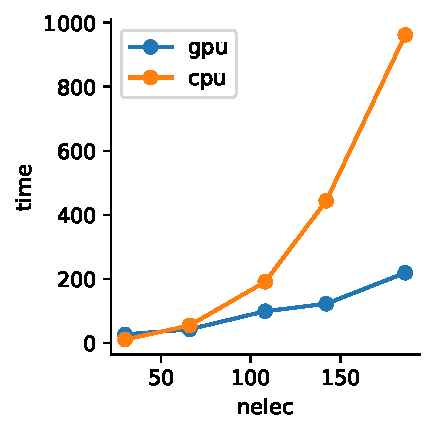
\includegraphics{figures/gpuplot.pdf}
\end{minipage}
\end{minipage}
\end{frame}


% 8. Conclusion
% flexible, all-python code
% active development, new features and optimizations
% available on github and pypi


\begin{frame}{Going forward}

\vspace{1em}

What we have now

\begin{itemize}[leftmargin=1em]
\item VMC, DMC, and optimization of ground and excited states
\item Working GPU implementation using CuPy

\quad Same code for CPU or GPU calculations
\item Integrated into PySCF
\end{itemize}

\vspace{1em}

What we can do with GPUs

\begin{itemize}[leftmargin=1em]
\item Leveraging GPU resources on supercomputers
\item Benchmark studies on molecules (ground/excited states)
\item Further optimization to speed up periodic calculations
\end{itemize}


\footnotesize{
% Citations
}

\end{frame}
